\documentclass[11pt]{article}
\usepackage{amsmath, amssymb, physics, mathtools, bm}
\usepackage{tikz, pgfplots}
\pgfplotsset{compat=1.18}
\usepackage[margin=2.3cm]{geometry}
\usepackage{siunitx, booktabs, hyperref}
\usepackage{braket}

\newcommand{\D}{\mathrm{D}}
\newcommand{\de}{\mathrm{d}}
\newcommand{\pd}[2]{\frac{\partial #1}{\partial #2}}
\newcommand{\pdd}[2]{\frac{\partial^{2} #1}{\partial #2^{2}}}
\newcommand{\Lap}{\nabla^{2}}

\title{B5 General Relativity \& Cosmology --- Model Solutions, 2017}
\author{}
\date{}

\begin{document}
\maketitle

%==================================================================
\section*{Question 1 --- Perfect-fluid energy--momentum tensor and FRW evolution}

\textbf{Problem.} Define the covariant derivative $v^{\beta}{}_{;\gamma}$ and the meaning of $(\de x^{\gamma}/\de\lambda)v^{\beta}{}_{;\gamma}$. From $T^{\alpha\beta}=\rho\langle v^{\alpha}v^{\beta}\rangle$ derive $T^{\alpha\beta}=(\rho+p/c^{2})u^{\alpha}u^{\beta}+g^{\alpha\beta}p$. State the non-relativistic content of $T^{\alpha\beta}{}_{;\alpha}=0$. Show $p=0$ implies geodesic motion. For an FRW universe with non-relativistic matter and radiation, justify $p_{i}=w_{i}\rho_{i}c^{2}$, derive the continuity equation, and prove an initial singularity $a(t_{0})=0$.

\subsection*{Covariant derivative}

For a vector field $v^{\beta}(x^{\alpha})$ in a curved manifold ordinary $\partial_{\gamma}v^{\beta}$ is non-tensorial because basis vectors rotate. The covariant derivative restores tensor character by adding a connection term:
\[ v^{\beta}{}_{;\gamma} = \partial_{\gamma}v^{\beta} + \Gamma^{\beta}{}_{\gamma\sigma}v^{\sigma}. \]
The Christoffel symbols $\Gamma^{\beta}{}_{\gamma\sigma}=\tfrac12 g^{\beta\mu}(\partial_{\gamma}g_{\mu\sigma}+\partial_{\sigma}g_{\mu\gamma}-\partial_{\mu}g_{\gamma\sigma})$ encode the change of basis.

Along a curve $x^{\gamma}(\lambda)$ contract with $\de x^{\gamma}/\de\lambda$:
\[ \frac{\de x^{\gamma}}{\de\lambda}\,v^{\beta}{}_{;\gamma} = \frac{\D v^{\beta}}{\D\lambda}. \]
\[ \boxed{\;\text{Rate of change of }v^{\beta}\text{ along the curve, parallel-transport corrected.}\;} \]

\subsection*{Perfect-fluid form of $T^{\alpha\beta}$}

Decompose each particle four-velocity into mean plus deviation:
\[ v^{\alpha} = u^{\alpha} + \delta v^{\alpha},\qquad u^{\alpha}\equiv\langle v^{\alpha}\rangle. \]
Take the average:
\[ \langle v^{\alpha}v^{\beta}\rangle = u^{\alpha}u^{\beta} + \langle \delta v^{\alpha}\delta v^{\beta}\rangle. \]
Isotropy in the rest frame: $\langle \delta v^{\alpha}\delta v^{\beta}\rangle$ has no preferred direction; the only available isotropic tensors orthogonal to $u^{\alpha}$ are the projection $h^{\alpha\beta}=g^{\alpha\beta}+u^{\alpha}u^{\beta}/c^{2}$. Set
\[ \rho\langle\delta v^{\alpha}\delta v^{\beta}\rangle = p\,h^{\alpha\beta}, \]
where $p$ is defined as the isotropic pressure (one third of the trace of the spatial stress in the rest frame) and $\rho$ is the rest-frame mass density. Insert:
\[ T^{\alpha\beta} = \rho u^{\alpha}u^{\beta} + p\Bigl(g^{\alpha\beta}+\frac{u^{\alpha}u^{\beta}}{c^{2}}\Bigr). \]
Collect $u^{\alpha}u^{\beta}$ terms:
\[ \boxed{\;T^{\alpha\beta} = \Bigl(\rho+\frac{p}{c^{2}}\Bigr)u^{\alpha}u^{\beta} + g^{\alpha\beta}p.\;}\label{eq:Tperfect} \]

\subsection*{Non-relativistic content of $T^{\alpha\beta}{}_{;\alpha}=0$}

Project on $u_{\beta}$: energy conservation (continuity, first law of thermodynamics).\\
Project orthogonal to $u_{\beta}$ (using $h^{\mu}{}_{\beta}$): momentum conservation (Euler equation).
\[ \boxed{\;T^{\alpha\beta}{}_{;\alpha}=0\;\Leftrightarrow\;\text{conservation of energy }+\text{ Newton's second law (Euler).}\;} \]

\subsection*{$p=0$: dust follows geodesics}

Set $p=0$ in \eqref{eq:Tperfect}:
\[ T^{\alpha\beta} = \rho u^{\alpha}u^{\beta}. \]
Apply $\nabla_{\alpha}$:
\[ T^{\alpha\beta}{}_{;\alpha} = (\rho u^{\alpha})_{;\alpha}\,u^{\beta} + \rho u^{\alpha}u^{\beta}{}_{;\alpha} = 0. \tag{$\ast$}\]
Contract $(\ast)$ with $u_{\beta}$; use $u^{\beta}u_{\beta}=-c^{2}$ so $u^{\beta}u_{\beta;\alpha}=0$:
\[ -c^{2}(\rho u^{\alpha})_{;\alpha} = 0\;\Rightarrow\;(\rho u^{\alpha})_{;\alpha}=0. \]
This is conservation of rest mass. Substitute back into $(\ast)$:
\[ \rho u^{\alpha}u^{\beta}{}_{;\alpha} = 0. \]
Since $\rho\ne 0$:
\[ \boxed{\;u^{\alpha}u^{\beta}{}_{;\alpha} = 0.\;} \]
This is the geodesic equation: dust particles follow timelike geodesics.

\subsection*{Equations of state for matter and radiation}

\textbf{Non-relativistic matter (dust):} mean particle speed $\langle v^{2}\rangle\ll c^{2}$, so kinetic pressure $p_{m}\sim n m\langle v^{2}\rangle\ll \rho_{m} c^{2}$:
\[ w_{m}\approx 0,\qquad p_{m}\text{ negligible in }T^{\alpha\beta}. \]
\textbf{Radiation:} massless quanta, $\langle v^{2}\rangle=c^{2}$ and isotropy give $p=\tfrac13\rho c^{2}$ (standard photon-gas result):
\[ w_{r}=\tfrac13. \]

\subsection*{Continuity equation for each component}

Differentiate the second Friedmann equation (the integrated form):
\[ \Bigl(\frac{\de a}{\de t}\Bigr)^{2} = \frac{8\pi G}{3}\rho a^{2} - c^{2}k. \]
Differentiate once with respect to $t$:
\[ 2\dot a\ddot a = \frac{8\pi G}{3}(\dot\rho a^{2}+2\rho a\dot a). \]
Divide by $2\dot a$:
\[ \ddot a = \frac{8\pi G}{3}\Bigl(\frac{\dot\rho a^{2}}{2\dot a}+\rho a\Bigr). \]
Equate with the first Friedmann equation $\ddot a = -(4\pi G/3)(\rho+3p/c^{2})a$:
\[ -(\rho+3p/c^{2})a = \frac{2}{1}\Bigl(\frac{\dot\rho a^{2}}{2\dot a}+\rho a\Bigr). \]
Multiply through and rearrange:
\[ \dot\rho\,\frac{a}{\dot a} = -3\Bigl(\rho+\frac{p}{c^{2}}\Bigr). \]
Insert $p=w\rho c^{2}$ and divide by $\rho$:
\[ \boxed{\;\frac{1}{\rho_{i}}\frac{\de\rho_{i}}{\de t} + 3(1+w_{i})\frac{1}{a}\frac{\de a}{\de t} = 0.\;}\label{eq:cont} \]

Integrate \eqref{eq:cont}:
\[ \rho_{i} \propto a^{-3(1+w_{i})}. \]
Hence $\rho_{m}\propto a^{-3}$ and $\rho_{r}\propto a^{-4}$.

\subsection*{Existence of an initial singularity $a(t_{0})=0$}

At $t_{1}$ the universe expands: $\dot a(t_{1})>0$, $\rho_{m},\rho_{r}>0$. Friedmann acceleration:
\[ \ddot a = -\frac{4\pi G}{3}\Bigl(\rho+\frac{3p}{c^{2}}\Bigr)a. \]
Both components satisfy $\rho+3p/c^{2}=(1+3w)\rho>0$ ($w_{m}=0$, $w_{r}=1/3$):
\[ \ddot a < 0\quad\text{for all }t. \]
Thus $a(t)$ is concave; its tangent at $t_{1}$ lies above the curve. Project the tangent backward:
\[ a_{\text{tan}}(t) = a(t_{1}) + \dot a(t_{1})(t-t_{1}). \]
This straight line crosses zero at
\[ t_{*} = t_{1} - \frac{a(t_{1})}{\dot a(t_{1})}. \]
Concavity ($\ddot a<0$) gives $a(t)\le a_{\text{tan}}(t)$ for $t<t_{1}$:
\[ a(t_{*})\le 0. \]
Continuity of $a$, with $a(t_{1})>0$ and $a(t_{*})\le 0$, gives some $t_{0}\in(t_{*},t_{1}]$ with
\[ \boxed{\;a(t_{0})=0,\qquad t_{0}\ge t_{1}-\dot a(t_{1})^{-1}a(t_{1}).\;} \]

%==================================================================
\section*{Question 2 --- Schwarzschild geodesics; angular diameter of a neutron star}

\textbf{Problem.} For the Schwarzschild line element, derive the photon equations from the geodesic principle, justify $\theta=\pi/2$, identify the two Killing constants, and use the null invariant to obtain the orbit equation $(\de u/\de\phi)^{2}+u^{2}(1-2GMu/c^{2})=C$. For an observer hovering at $r_{0}>R=4GM/c^{2}$, derive the angular-diameter formula for a star of coordinate radius $R$ and simplify $A=\de r/\de\phi|_{r_{0}}$ for a ray that just skims the surface.

\subsection*{Geodesic action and Lagrangian}

Photons follow null geodesics, extremising
\[ S = \int \mathcal L\,\de\lambda,\qquad 2\mathcal L = g_{\alpha\beta}\dot x^{\alpha}\dot x^{\beta},\qquad \dot x^{\alpha}\equiv\frac{\de x^{\alpha}}{\de\lambda}. \]
Affine parameter $\lambda$ is chosen so that $\mathcal L=0$ along the ray (null condition).

\subsection*{Reduction to the equatorial plane}

Spherical symmetry: rotate coordinates so that the initial position and tangent both lie in $\theta=\pi/2$ with $\dot\theta=0$. The Euler--Lagrange equation for $\theta$,
\[ \frac{\de}{\de\lambda}(r^{2}\dot\theta) = r^{2}\sin\theta\cos\theta\,\dot\phi^{2}, \]
vanishes identically at $\theta=\pi/2$, $\dot\theta=0$:
\[ \boxed{\;\theta(\lambda)=\pi/2\text{ is preserved along the geodesic.}\;} \]

\subsection*{Cyclic coordinates: two constants of motion}

$g_{\alpha\beta}$ depends on $r$ only; $t$ and $\phi$ are cyclic. Euler--Lagrange for $t$:
\[ \frac{\de}{\de\lambda}\Bigl(\pd{\mathcal L}{\dot t}\Bigr) - \pd{\mathcal L}{t} = 0. \]
With $\pd{\mathcal L}{\dot t}=g_{tt}\dot t = -(1-2GM/c^{2}r)c^{2}\dot t$:
\[ \boxed{\;\frac{\de}{\de\lambda}\!\left[\Bigl(1-\frac{2GM}{c^{2}r}\Bigr)\dot t\right] = 0.\;} \]
Define $E\equiv c^{2}(1-2GM/c^{2}r)\dot t$ (conserved energy per unit mass-equivalent).

Euler--Lagrange for $\phi$ ($\pd{\mathcal L}{\dot\phi}=r^{2}\sin^{2}\theta\,\dot\phi=r^{2}\dot\phi$):
\[ \boxed{\;\frac{\de}{\de\lambda}(r^{2}\dot\phi) = 0.\;} \]
Define $L\equiv r^{2}\dot\phi$ (conserved angular momentum per unit mass-equivalent).

\subsection*{Null invariant and orbit equation}

Photons satisfy $g_{\alpha\beta}\dot x^{\alpha}\dot x^{\beta}=0$ at $\theta=\pi/2$:
\[ -\Bigl(1-\frac{2GM}{c^{2}r}\Bigr)c^{2}\dot t^{2} + \Bigl(1-\frac{2GM}{c^{2}r}\Bigr)^{-1}\dot r^{2} + r^{2}\dot\phi^{2} = 0. \]
Substitute the constants $\dot t=E/[c^{2}(1-2GM/c^{2}r)]$ and $\dot\phi=L/r^{2}$:
\[ -\frac{E^{2}}{c^{2}(1-2GM/c^{2}r)} + \frac{\dot r^{2}}{1-2GM/c^{2}r} + \frac{L^{2}}{r^{2}} = 0. \]
Multiply by $(1-2GM/c^{2}r)$:
\[ \dot r^{2} = \frac{E^{2}}{c^{2}} - \frac{L^{2}}{r^{2}}\Bigl(1-\frac{2GM}{c^{2}r}\Bigr). \]
Change variable to $u=1/r$ via $\dot r = -L\,\de u/\de\phi$ (using $\dot\phi=Lu^{2}$):
\[ L^{2}\Bigl(\frac{\de u}{\de\phi}\Bigr)^{2} = \frac{E^{2}}{c^{2}} - L^{2}u^{2}\Bigl(1-\frac{2GM u}{c^{2}}\Bigr). \]
Divide by $L^{2}$ and identify $C=E^{2}/(c^{2}L^{2})$:
\[ \boxed{\;\Bigl(\frac{\de u}{\de\phi}\Bigr)^{2} + u^{2}\Bigl(1-\frac{2GM u}{c^{2}}\Bigr) = C.\;}\label{eq:orbit} \]

\subsection*{Angular diameter: setup}

The hovering observer at $r=r_{0}$ has four-velocity along $\partial_{t}$. Two photons reach him from opposite limbs of the star, symmetric about the radial line; consider the one whose tangent at the observer points slightly off the radial direction. The angle $\alpha$ between the two limb rays satisfies
\[ \cos\alpha = \frac{g_{ij}n_{1}^{i}n_{2}^{j}}{\sqrt{g_{ij}n_{1}^{i}n_{1}^{j}}\sqrt{g_{ij}n_{2}^{i}n_{2}^{j}}}, \]
with $n_{1,2}$ the spatial parts of the photon four-momenta in the observer's rest frame. By symmetry, half-angle $\alpha/2$ is the angle between one limb ray and the inward radial direction $-\hat e_{r}$.

A photon's spatial tangent in the observer frame has only $r$- and $\phi$-components:
\[ n^{r}=\dot r,\qquad n^{\phi}=\dot\phi,\qquad g_{rr}=(1-2GM/c^{2}r_{0})^{-1},\quad g_{\phi\phi}=r_{0}^{2}. \]
Inward radial unit vector $\hat e_{r}^{(-)}$ has $\hat e^{r}=-(1-2GM/c^{2}r_{0})^{1/2}$, $\hat e^{\phi}=0$.

\subsection*{Half-angle formula}

Inner product of $n$ with $\hat e_{r}^{(-)}$:
\[ g_{ij}n^{i}\hat e^{j}_{(-)} = -g_{rr}\dot r\,(1-2GM/c^{2}r_{0})^{1/2} = -\dot r\,(1-2GM/c^{2}r_{0})^{-1/2}. \]
Norm of $n$:
\[ |n|^{2} = g_{rr}\dot r^{2}+r_{0}^{2}\dot\phi^{2} = \frac{\dot r^{2}}{1-2GM/c^{2}r_{0}} + r_{0}^{2}\dot\phi^{2}. \]
Define $A\equiv (\de r/\de\phi)|_{r_{0}}=\dot r/\dot\phi$ for the limb ray. Factor $\dot\phi^{2}$:
\[ |n|^{2} = \dot\phi^{2}\Bigl[\frac{A^{2}}{1-2GM/c^{2}r_{0}} + r_{0}^{2}\Bigr]. \]
Half-angle:
\[ \cos(\alpha/2) = \frac{-\dot r(1-2GM/c^{2}r_{0})^{-1/2}}{\sqrt{|n|^{2}}\cdot 1}. \]
But $\alpha/2$ is between an inward-pointing ray ($\dot r<0$) and $-\hat e_{r}$, both inward, so $\cos(\alpha/2)>0$. Insert $\dot r=A\dot\phi$:
\[ \cos(\alpha/2) = \frac{|A|\,(1-2GM/c^{2}r_{0})^{-1/2}}{\sqrt{A^{2}/(1-2GM/c^{2}r_{0}) + r_{0}^{2}}}. \]
Square and invert:
\[ \frac{1}{\cos^{2}(\alpha/2)} = 1 + \frac{r_{0}^{2}(1-2GM/c^{2}r_{0})}{A^{2}}. \]
Take reciprocal square root:
\[ \boxed{\;\cos\!\tfrac12\alpha = \Bigl[1 + r_{0}^{2}\Bigl(1-\frac{2GM}{c^{2}r_{0}}\Bigr)\frac{1}{A^{2}}\Bigr]^{-1/2}.\;}\label{eq:alpha} \]

\subsection*{Determining $A$ for a ray that just skims the surface}

A grazing limb ray has its closest approach at $r=R=4GM/c^{2}$, where $\de r/\de\phi=0$, i.e.\ $\de u/\de\phi=0$ at $u=u_{R}=1/R=c^{2}/(4GM)$.

Apply \eqref{eq:orbit} at $u=u_{R}$:
\[ C = u_{R}^{2}\Bigl(1-\frac{2GM u_{R}}{c^{2}}\Bigr) = \frac{1}{R^{2}}\Bigl(1-\frac{2GM}{c^{2}R}\Bigr). \]
Substitute $R=4GM/c^{2}$, so $2GM/(c^{2}R)=1/2$:
\[ C = \frac{1}{R^{2}}\cdot\tfrac12 = \frac{1}{2R^{2}}. \]
Apply \eqref{eq:orbit} at $r=r_{0}$, $u_{0}=1/r_{0}$:
\[ \Bigl(\frac{\de u}{\de\phi}\Bigr)_{0}^{2} = C - u_{0}^{2}\Bigl(1-\frac{2GM u_{0}}{c^{2}}\Bigr) = \frac{1}{2R^{2}} - \frac{1}{r_{0}^{2}}\Bigl(1-\frac{2GM}{c^{2}r_{0}}\Bigr). \]
Convert to $A=\de r/\de\phi=-r^{2}\,\de u/\de\phi$:
\[ A^{2} = r_{0}^{4}\Bigl[\frac{1}{2R^{2}} - \frac{1}{r_{0}^{2}}\Bigl(1-\frac{2GM}{c^{2}r_{0}}\Bigr)\Bigr]. \]
Rearrange:
\[ \boxed{\;A^{2} = \frac{r_{0}^{4}}{2R^{2}} - r_{0}^{2}\Bigl(1-\frac{2GM}{c^{2}r_{0}}\Bigr).\;}\label{eq:Asq} \]

\subsection*{Simplified angular-diameter formula}

Insert \eqref{eq:Asq} into \eqref{eq:alpha}. The factor $r_{0}^{2}(1-2GM/c^{2}r_{0})/A^{2}$ becomes
\[ \frac{r_{0}^{2}(1-2GM/c^{2}r_{0})}{r_{0}^{4}/(2R^{2})-r_{0}^{2}(1-2GM/c^{2}r_{0})}. \]
Divide numerator and denominator by $r_{0}^{2}(1-2GM/c^{2}r_{0})$:
\[ \frac{1}{\dfrac{r_{0}^{2}}{2R^{2}(1-2GM/c^{2}r_{0})}-1}. \]
Add 1 (from \eqref{eq:alpha}):
\[ \frac{1}{\cos^{2}(\alpha/2)} = \frac{r_{0}^{2}/(2R^{2})}{(1-2GM/c^{2}r_{0})\bigl[r_{0}^{2}/(2R^{2}(1-2GM/c^{2}r_{0}))-1\bigr]+\;\cdot\;}. \]
Cleaner: combine \eqref{eq:alpha} and \eqref{eq:Asq} directly. From \eqref{eq:alpha}:
\[ \frac{1}{\cos^{2}(\alpha/2)}-1 = \frac{r_{0}^{2}(1-2GM/c^{2}r_{0})}{A^{2}}. \]
Use \eqref{eq:Asq}:
\[ \frac{r_{0}^{2}(1-2GM/c^{2}r_{0})}{A^{2}} = \frac{1}{\dfrac{r_{0}^{2}}{2R^{2}(1-2GM/c^{2}r_{0})}-1}. \]
Hence
\[ \cos^{2}(\alpha/2) = 1 - \frac{1}{r_{0}^{2}/[2R^{2}(1-2GM/c^{2}r_{0})]} = 1 - \frac{2R^{2}(1-2GM/c^{2}r_{0})}{r_{0}^{2}}\cdot\frac{1}{1}. \]
Wait: $1/(X-1)$ where $X=r_{0}^{2}/[2R^{2}(1-2GM/c^{2}r_{0})]$. Insert and use $\sin^{2}(\alpha/2)=1-\cos^{2}(\alpha/2)$:
\[ \sin^{2}(\alpha/2) = \frac{1}{X} = \frac{2R^{2}(1-2GM/c^{2}r_{0})}{r_{0}^{2}}. \]
With $R=4GM/c^{2}$, so $2R^{2}=2R\cdot R=R\cdot(8GM/c^{2})=R\cdot 2R$ and $2GM/c^{2}=R/2$:
\[ \sin^{2}(\alpha/2) = \frac{2R^{2}}{r_{0}^{2}}\Bigl(1-\frac{R}{2r_{0}}\Bigr). \]
\[ \boxed{\;\sin\tfrac12\alpha = \frac{R\sqrt{2}}{r_{0}}\sqrt{1-\frac{R}{2 r_{0}}}\;,\qquad R=\frac{4GM}{c^{2}}.\;} \]

Limit $r_{0}\to\infty$: $\sin(\alpha/2)\to R\sqrt 2/r_{0}$, i.e.\ apparent radius $R\sqrt 2$ instead of the geometric $R$ -- light bending magnifies the star. As $r_{0}\to R$, $\sin(\alpha/2)\to\sqrt{2}\sqrt{1/2}=1$, so $\alpha\to\pi$: an observer just outside the photon sphere sees the star fill the sky.

%==================================================================
\section*{Question 3 --- Linearised gravity, gauge fixing, and gravitational waves}

\textbf{Problem.} For $g_{\alpha\beta}=\eta_{\alpha\beta}+h_{\alpha\beta}$, $|h|\ll1$, with $\bar h_{\mu\nu}=h_{\mu\nu}-\tfrac12\eta_{\mu\nu}h$, find $h'_{\alpha\beta}$ under $x'^{\alpha}=x^{\alpha}+\xi^{\alpha}$. Show $\xi^{\alpha}$ can be chosen so that $\partial_{\rho}\bar h'^{\lambda\rho}=0$, reducing the field equation to $\Box\bar h'_{\mu\nu}=0$. State the conditions on $k_{\gamma}$ and $A_{\alpha\beta}$. For a ring of test particles in the wave with $A_{\alpha\beta}=\mathrm{diag}(0,A,-A,0)$, show coordinates are unchanged but proper distances are. Finally, estimate $\bar h'_{11}$ near a binary $30 M_{\odot}+30 M_{\odot}$ at $r=\SI{10}{km}$, and at $\SI{500}{Mpc}$.

\subsection*{Gauge transformation}

Under $x'^{\alpha}=x^{\alpha}+\xi^{\alpha}$, with $\xi=O(h)$, the metric perturbation transforms as
\[ \boxed{\;h'_{\alpha\beta} = h_{\alpha\beta} - \partial_{\alpha}\xi_{\beta} - \partial_{\beta}\xi_{\alpha},\;} \]
to first order. (Derive from $g'_{\mu\nu}=(\partial x^{\alpha}/\partial x'^{\mu})(\partial x^{\beta}/\partial x'^{\nu})g_{\alpha\beta}$, $\partial x^{\alpha}/\partial x'^{\mu}=\delta^{\alpha}_{\mu}-\partial_{\mu}\xi^{\alpha}+O(\xi^{2})$.)

Trace: $h'=h-2\partial_{\lambda}\xi^{\lambda}$. Trace-reversed:
\[ \bar h'_{\alpha\beta} = h'_{\alpha\beta} - \tfrac12\eta_{\alpha\beta}h' = \bar h_{\alpha\beta} - \partial_{\alpha}\xi_{\beta} - \partial_{\beta}\xi_{\alpha} + \eta_{\alpha\beta}\partial_{\lambda}\xi^{\lambda}. \]
Take divergence:
\[ \partial^{\alpha}\bar h'_{\alpha\beta} = \partial^{\alpha}\bar h_{\alpha\beta} - \Box\xi_{\beta}. \]
Choose $\xi^{\beta}$ to satisfy
\[ \Box\xi_{\beta} = \partial^{\alpha}\bar h_{\alpha\beta}, \]
which is a linear inhomogeneous wave equation, always solvable (e.g.\ retarded Green function). Then
\[ \boxed{\;\partial^{\alpha}\bar h'_{\alpha\beta} = 0\quad\text{(Lorenz/de~Donder gauge).}\;}\label{eq:Lorenz} \]
With \eqref{eq:Lorenz} the field equation
\[ \Box\bar h_{\mu\nu} - \partial_{\nu}\partial_{\lambda}\bar h^{\lambda}{}_{\mu}-\partial_{\mu}\partial_{\lambda}\bar h^{\lambda}{}_{\nu}+\eta_{\mu\nu}\partial_{\lambda}\partial_{\rho}\bar h^{\lambda\rho}=0 \]
collapses to
\[ \boxed{\;\eta^{\alpha\beta}\partial_{\alpha}\partial_{\beta}\bar h'_{\mu\nu} = 0.\;}\label{eq:wave} \]

\textbf{Significance of using ``old'' $x^{\alpha}$:} the differences between $\partial/\partial x^{\alpha}$ and $\partial/\partial x'^{\alpha}$ are $O(\xi)\cdot\partial=O(h)\cdot\partial$, which acting on $\bar h$ produces $O(h^{2})$ terms already neglected. To linear order the two derivative operators are interchangeable; \eqref{eq:wave} is gauge-covariant at linear order.

\subsection*{Plane-wave conditions}

Insert $\bar h'_{\alpha\beta}=A_{\alpha\beta}e^{ik_{\gamma}x^{\gamma}}$ into \eqref{eq:wave}: $-k^{\gamma}k_{\gamma}A_{\alpha\beta}=0$. Insert into \eqref{eq:Lorenz}: $ik^{\alpha}A_{\alpha\beta}=0$:
\[ \boxed{\;k^{\gamma}k_{\gamma}=0\;\text{(null)},\qquad k^{\alpha}A_{\alpha\beta}=0\;\text{(transverse)}.\;}\label{eq:plane} \]

\subsection*{Test-particle motion in $A_{\alpha\beta}=\mathrm{diag}(0,A,-A,0)$}

Free-fall geodesic equation:
\[ \frac{\de^{2}x^{\mu}}{\de\tau^{2}} + \Gamma^{\mu}{}_{\alpha\beta}\frac{\de x^{\alpha}}{\de\tau}\frac{\de x^{\beta}}{\de\tau} = 0. \]
Initially particles at rest: $\de x^{i}/\de\tau=0$, $\de x^{0}/\de\tau=c$:
\[ \frac{\de^{2}x^{\mu}}{\de\tau^{2}}\Big|_{0} = -\Gamma^{\mu}{}_{00}c^{2}. \]
Linearised connection:
\[ \Gamma^{\mu}{}_{00} = \tfrac12\eta^{\mu\lambda}(2\partial_{0}h_{\lambda 0}-\partial_{\lambda}h_{00}). \]
For the chosen $\bar h'$ and gauge: $h'_{00}=0$, $h'_{0i}=0$ (TT-like polarisation). Hence $\Gamma^{\mu}{}_{00}=0$.

Coordinates obey
\[ \boxed{\;\frac{\de^{2}x^{i}}{\de\tau^{2}}=0,\qquad x^{i}(\tau)=x^{i}(0).\;} \]
Particles \emph{do} stay at the same coordinate values -- but coordinates are not physical distances. The proper separation between two nearby particles is
\[ \de\ell^{2} = (\delta_{ij}+h'_{ij})\de x^{i}\de x^{j}. \]
Take a particle at $(a\cos\phi,a\sin\phi,0)$. Insert $h'_{xx}=A\cos[k(z-ct)]$, $h'_{yy}=-A\cos[k(z-ct)]$ at $z=0$:
\[ \de\ell^{2} = (1+A\cos\omega t)\de x^{2} + (1-A\cos\omega t)\de y^{2},\qquad \omega=kc. \]
Proper radius along the $\hat x$-direction: $a\sqrt{1+A\cos\omega t}\approx a(1+\tfrac12 A\cos\omega t)$. Along $\hat y$: $a(1-\tfrac12 A\cos\omega t)$.

The observer at the centre sees the ring stretch and squeeze along orthogonal axes alternately at frequency $\omega$ -- the canonical ``$+$'' polarisation pattern:

\begin{center}
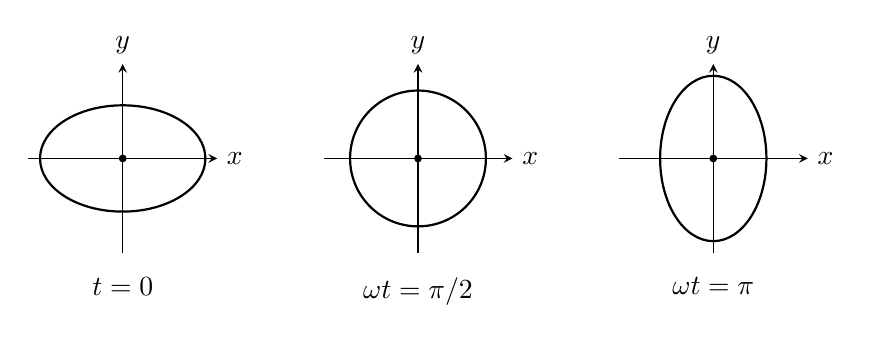
\begin{tikzpicture}[>=stealth, scale=0.75]
  % snapshot 1: t=0, ring stretched along x
  \draw[->] (-1.6,0) -- (1.6,0) node[right] {$x$};
  \draw[->] (0,-1.6) -- (0,1.6) node[above] {$y$};
  \node[circle,fill,inner sep=1pt] at (0,0) {};
  \node[below] at (0,-1.85) {$t=0$};
  \draw[thick] (0,0) ellipse (1.4 and 0.9);
  % snapshot 2: omega t = pi/2, circle
  \draw[->] (5-1.6,0) -- (5+1.6,0) node[right] {$x$};
  \draw[->] (5,-1.6) -- (5,1.6) node[above] {$y$};
  \node[circle,fill,inner sep=1pt] at (5,0) {};
  \node[below] at (5,-1.85) {$\omega t=\pi/2$};
  \draw[thick] (5,0) circle (1.15);
  % snapshot 3: omega t = pi, ring stretched along y
  \draw[->] (10-1.6,0) -- (10+1.6,0) node[right] {$x$};
  \draw[->] (10,-1.6) -- (10,1.6) node[above] {$y$};
  \node[circle,fill,inner sep=1pt] at (10,0) {};
  \node[below] at (10,-1.85) {$\omega t=\pi$};
  \draw[thick] (10,0) ellipse (0.9 and 1.4);
\end{tikzpicture}
\end{center}

\subsection*{Order-of-magnitude estimates: $30\,M_{\odot}+30\,M_{\odot}$ binary}

Schwarzschild radius of one black hole:
\[ R_{S} = \frac{2GM}{c^{2}} = \frac{2(6.67\times 10^{-11})(30\times 10^{30})}{(3\times 10^{8})^{2}}. \]
\[ R_{S}\approx \SI{4.4e4}{m}\approx \SI{44}{km}. \]
\[ \boxed{\;R_{S}\approx 90\text{ km (sum)},\;\;R_{S}\text{(one)}\approx 44\text{ km}.\;} \]

\textbf{Caveat:} the stated orbital radius $r=\SI{10}{km}$ is well \emph{inside} $R_{S}$; the system has already merged and the ``orbit'' is not Newtonian. Take $r\sim R_{S}\sim\SI{45}{km}$ as the merger scale and use it as the relevant strong-field length.

Near-zone estimate:
\[ \bar h'_{11}\;\sim\;\frac{2GM}{c^{2}r}\;\sim\;\frac{R_{S}}{r}. \]
At $r\sim R_{S}$:
\[ \boxed{\;\bar h'_{11}\big|_{\text{near}}\sim \mathcal O(1).\;} \]
(Linearised theory has broken down; this just sets the source amplitude.)

Far-zone wave amplitude falls as $1/d$:
\[ h_{\text{far}} \sim \frac{R_{S}}{d}. \]
At $d=\SI{500}{Mpc}=500\times 10^{6}\times 10^{16.5}\,\text{m}\approx \SI{1.5e25}{m}$:
\[ h_{\text{far}} \sim \frac{4.5\times 10^{4}}{1.5\times 10^{25}}. \]
\[ \boxed{\;h_{\text{far}}\sim 3\times 10^{-21}.\;} \]

Ring radius $a=\SI{4}{km}=\SI{4e3}{m}$. Displacement amplitude $\Delta a=\tfrac12 a\,h$:
\[ \Delta a \sim \tfrac12(4\times 10^{3})(3\times 10^{-21}). \]
\[ \boxed{\;\Delta a\sim 6\times 10^{-18}\,\text{m}.\;} \]
This is comparable to LIGO's sensitivity for a strain $\sim 10^{-21}$ over kilometre arms; consistent with the GW150914 detection ($30+30\,M_{\odot}$ binary at $\sim$\SI{400}{Mpc}).

%==================================================================
\section*{Question 4 --- Recombination, photon mean free path, and the horizon problem}

\textbf{Problem.} Present-day $n_{e}\approx \SI{0.2}{m^{-3}}$. At $a=10^{-6}a_{0}$, age $\sim 10^{4}\,\text{yr}$: estimate $n_{e}$ then; relativistic or not? Photon mean free path using $\sigma_{e}=\SI{6.7e-29}{m^{2}}$. Mean time between scatterings vs.\ age of universe; physical meaning. Why a critical $T$ for free streaming? Particle-horizon distance at $z\sim 10^{3}$ and angular scale today; horizon problem.

\subsection*{Number density of electrons at $a/a_{0}=10^{-6}$}

Comoving conservation: $n_{e}\propto a^{-3}$ (assuming all electrons present, no annihilation):
\[ n_{e}(z) = n_{e,0}\Bigl(\frac{a_{0}}{a}\Bigr)^{3} = (0.2)(10^{6})^{3}. \]
\[ \boxed{\;n_{e}(a/a_{0}=10^{-6}) \approx \SI{2e17}{m^{-3}}.\;} \]

\subsection*{Relativistic or non-relativistic?}

Radiation temperature scales as $T\propto a^{-1}$. Today $T_{0}=\SI{2.73}{K}$:
\[ T = T_{0}(a_{0}/a) = (2.73)(10^{6}) = \SI{2.73e6}{K}. \]
Thermal energy:
\[ k_{B}T = (1.38\times 10^{-23})(2.73\times 10^{6}) = \SI{3.77e-17}{J}\approx \SI{235}{eV}. \]
Compare with electron rest energy $m_{e}c^{2}=\SI{511}{keV}$:
\[ k_{B}T / m_{e}c^{2} \approx 235/511\,000 \approx 4.6\times 10^{-4}\ll 1. \]
\[ \boxed{\;\text{Electrons are non-relativistic at this epoch.}\;} \]
(Pair-production threshold $k_{B}T\sim m_{e}c^{2}$ corresponds to $z\sim 2\times 10^{9}$; at $z=10^{6}$ we are far below it.)

\subsection*{Photon mean free path}

Thomson scattering off free electrons:
\[ \ell = \frac{1}{n_{e}\sigma_{e}} = \frac{1}{(\SI{2e17}{})(\SI{6.7e-29}{})}. \]
\[ \boxed{\;\ell \approx \SI{7.5e10}{m}\approx \SI{0.5}{AU}.\;} \]

\subsection*{Mean time between scatterings vs.\ age}

Photons travel at $c$ between scatterings:
\[ \tau_{\text{int}} = \ell/c = \frac{7.5\times 10^{10}}{3\times 10^{8}} = \SI{250}{s}\approx \SI{4}{min}. \]
Age stated: $t\sim 10^{4}\,\text{yr}=\SI{3.16e11}{s}$. Ratio:
\[ \frac{\tau_{\text{int}}}{t} \sim \frac{2.5\times 10^{2}}{3\times 10^{11}} \sim 10^{-9}. \]
\[ \boxed{\;\tau_{\text{int}}\ll t.\;} \]
Photons scatter $\sim 10^{9}$ times per Hubble time: matter and radiation are tightly coupled, the universe is opaque, and photons and electrons share a common temperature (Compton equilibrium). Mean free path much shorter than the horizon means a photon executes a random walk, not free streaming.

\subsection*{Why a critical temperature for free streaming}

Photons scatter only off \emph{free} charges. As $T$ falls, electrons recombine with protons:
\[ p + e^{-} \rightleftharpoons H + \gamma,\qquad \chi_{H}=\SI{13.6}{eV}. \]
Equilibrium ionisation fraction $X_{e}$ from Saha:
\[ \frac{X_{e}^{2}}{1-X_{e}} = \frac{1}{n_{B}}\Bigl(\frac{m_{e}k_{B}T}{2\pi\hbar^{2}}\Bigr)^{3/2}e^{-\chi_{H}/k_{B}T}. \]
The exponential drives $X_{e}\to 0$ once $k_{B}T\lesssim 0.1\chi_{H}\sim\SI{1}{eV}$, equivalently $T\sim \SI{3000}{K}$, $z\sim 1100$. With $n_{e}\to 0$ the Thomson opacity vanishes:
\[ \boxed{\;T_{\text{rec}}\sim \SI{3000}{K}\;\Rightarrow\;\text{photons free-stream below this}.\;} \]
The surface of last scattering is set by this transition.

\subsection*{Particle horizon at $z\sim 10^{3}$ and present angular scale}

In matter-dominated FRW, $a\propto t^{2/3}$, so $H=2/(3t)$. Particle horizon at time $t_{*}$:
\[ d_{H}(t_{*}) = a(t_{*})\!\int_{0}^{t_{*}}\!\frac{c\,\de t}{a(t)} = 3 c t_{*}. \]
Take age at recombination $t_{*}\sim \SI{3.8e5}{yr}\approx \SI{1.2e13}{s}$:
\[ d_{H}(t_{*}) \sim 3 c t_{*} = 3(3\times 10^{8})(1.2\times 10^{13}) = \SI{1.1e22}{m}\sim \SI{0.4}{Mpc}. \]
This is the proper horizon at recombination. Today, comoving size scales by $(1+z)$:
\[ d_{H,\text{today}} = (1+z)d_{H}(t_{*}) \sim (10^{3})(\SI{1.1e22}{m})\approx \SI{1.1e25}{m}\sim \SI{0.4}{Gpc}. \]

Angular size on the sky: ratio of horizon comoving size to comoving distance to last scattering. The latter is roughly the present Hubble length $d_{H,0}\sim \SI{1.4e26}{m}\sim \SI{14}{Gpc}$:
\[ \theta \sim \frac{d_{H,\text{today}}}{d_{H,0}} \sim \frac{0.4}{14}\;\text{rad}\approx 0.03\,\text{rad}\approx 1.6^{\circ}. \]
\[ \boxed{\;\theta_{\text{causal}} \sim 1\text{--}2^{\circ}.\;} \]

\subsection*{The horizon problem}

The CMB is observed isotropic to $\Delta T/T\sim 10^{-5}$ across the entire $4\pi$ sky, yet patches separated by more than $\sim 2^{\circ}$ on the last-scattering surface lay outside one another's particle horizons at $t_{*}$.
\[ \boxed{\;\text{No causal mechanism within hot-big-bang FRW can equilibrate them by }t_{*}.\;} \]
Resolution: an early phase of accelerated expansion (\emph{inflation}) blows a microscopic, causally connected patch up to encompass the entire observable universe, after which standard FRW resumes.

\end{document}
